\documentclass[12pt]{article}
\usepackage[english]{babel}
\usepackage[utf8x]{inputenc}
\usepackage[T1]{fontenc}
\usepackage{lab}
\usepackage{listings}
\usepackage{comment}


\Instructors{Alex Mussa, Kevin Johnson}
\LabNumber{5}
\LabTitle{Analog and Digital Signal Processing}
\LabDate{July 10th, 2019}

\lstset{style=mystyle}

\begin{document}
\MakeLabTop

\section{Introduction}

The signals generated from devices such as sensors are sometimes corrupt with noise, need to have some math done to them to make them mean something, or be processed to make a decision from the information. In order to enable the microcontroller to input this information for computation, digital signal processing is necessary to convert the physical analog signal into a digital representation of what the voltage value is. It is also possible to manipulate signals with analog circuits such as RC filters. Similar effects of these devices can also be implemented digitally with digital filters once the signal is converted to a digital representation.

In this lab, we will explore some basic acquisition and signal processing topics, both analog and digital. Sampling an analog signal involves some parameters, such as resolution and sampling rate, which will be explored. The basic functionality of a RC low-pass filter will be explored and demonstrated on removing noise from a low-frequency signal. Additionally, you will write code to implement a moving average digital filter to also remove the noise, but with the arduino microcontroller. 

\section{Setup}

\subsection{Collecting the required materials}

\textbf{\underline{INSTRUCTIONS}}

\begin{enumerate}
    \item Collect four BNC to Alligator cables from the cable rack in the lab. Two for the waveform generator, two for the oscilloscope.
    \item Collect the following supplies from the instructors:
    \begin{enumerate}
        \item Arduino Nano Microcontroller
        \item Breadboard
        \item Wire
        \item .33 $\mu$F capacitor
        \item 4.7k$\Omega$ resistor
    \end{enumerate}
\end{enumerate}

\subsection{Capacitors}

A capacitor is a circuit element, similar to a resistor, that behaves in such a manner that the amount of resistance it contributes to a circuit depends on the frequency of the signal that is being sent through it.  Capacitance is measured in units of Farads (F), and the capacitance affects the effective resistance of the capacitor at different frequencies. Take for consideration the circuit image of the voltage divider and the resistor and capacitor in \textit{Figure 1}.

\begin{figure}[H]
\begin{subfigure}{.5\textwidth}
    \centering
    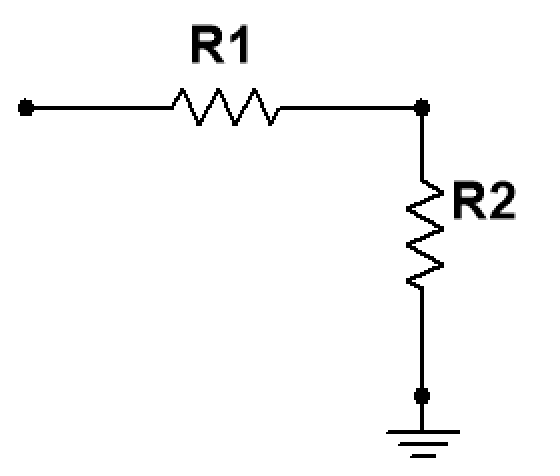
\includegraphics[width=0.8\linewidth]{photos/lab/voltagediv.png}
    \caption{A voltage divider circuit.}
\end{subfigure}%
\begin{subfigure}{.5\textwidth}
  \centering
  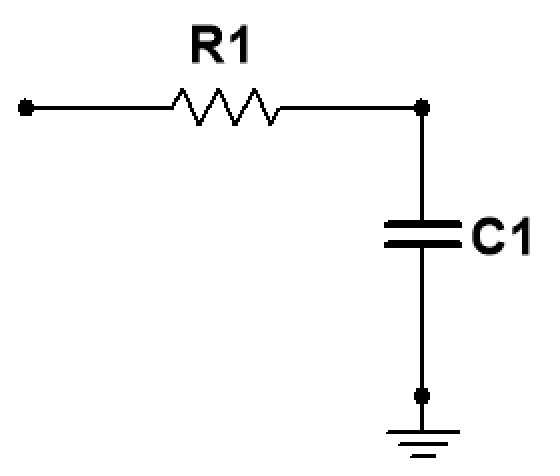
\includegraphics[width=0.79\linewidth]{photos/lab/RC.png}
  \caption{An RC lowpass filter.}
\end{subfigure}
\caption{Comparing a series resistor and capacitor to a voltage divider.}
\end{figure}

The voltage divider should seem familiar, as it is a series combination of resistances. Previously, we used ohms law to solve for the current through both of the series resistors, and used this to find the value of the voltage drop across the second resistor, R2, as $V_{2} = I * R_{2} = \frac{V}{R_{1} + R_{2}} * R_{2}$. A series of RC behaves similarly, except the "resistance" varies depending upon the following: $R_{C} = \frac{1}{\omega C}$. We can relate this to the resistance, as it can be seen in the previous equation that its value help determine how much of the signal is \textit{attenuated}, or made smaller. In reality, though, capacitor cause a delay in time for the signal to travel through it, causing a phase shift. For this reason, capacitors aren't refered to by their resistance, but by their \textit{impedance} as $Z = \frac{1}{j \omega C}$. For this class, we will neglect the phase shifting principle in our calculations and just focus on the attenuation of the signal.

To see how much attenuation would happen in the circuit in \textit{Figure 1 (b)} with values $R_{1} = 1k \Omega$ and $C_{1} = 1 mF$, with a sinusoid signal operating at a frequency of $f= \frac{1}{2\pi} Hz$, such that $\omega = 2\pi *f = 2\pi* \frac{1}{2\pi} = 1 \frac{radians}{sec}$. To begin, the effective resistance of the capacitor must be calculated as $R_{C} = \frac{1}{\omega C} = \frac{1}{1 * 1mF} = 1k\Omega$. This attenuation can be computed as a ratio with the above equation for the voltage in $R_{2}$ in the voltage divider, where $R_{2} = R_{C}$, with the exception that due to the true impedance being an imaginary number and having the $j=\sqrt{-1}$ which we will ignore completely in this class, the denominator changes from the previous such that $V_{C} = \frac{V}{\sqrt{R_{1}^{2} + R_{2}^{2}}} * R_{2} = \frac{V}{\sqrt{1k\Omega^{2} + 1k\Omega^{2}}} * 1k\Omega = 0.7071 * V$. If we refer to this voltage across the capacitor as the output voltage and the voltage across the resistor and capacitor, V, the peak-to-peak value of the input sinusoidal voltage, we can compute the ratio of the output to the input as $\frac{V_{out}}{V_{in}} = \frac{0.7071*V}{V} = 0.7071$. This frequency where the filter produces an attenuation of 0.7071 of the original amplitude is known as the cutoff frequency of the filter, and can be computed from the resistor and capacitors value as $f_{c} = \frac{1}{2\pi RC}$.

\begin{figure}[H]
\begin{subfigure}{.5\textwidth}
    \centering
    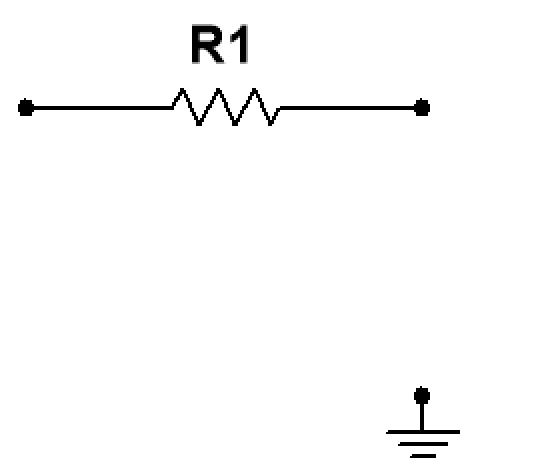
\includegraphics[width=0.8\linewidth]{photos/lab/open.png}
    \caption{RC Filters equivalent when frequency is very low.}
\end{subfigure}%
\begin{subfigure}{.5\textwidth}
  \centering
  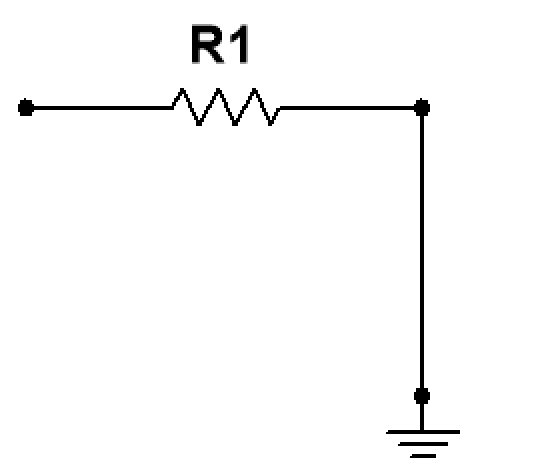
\includegraphics[width=0.79\linewidth]{photos/lab/short.png}
  \caption{RC Filters equivalent when frequency is very high.}
\end{subfigure}
\caption{Comparison of circuits operation at very high frequencies versus very low frequencies for a low-pass filter.}
\end{figure}

Considering the amount of resistance introduced by the capacitor as $R_{C} = \frac{1}{\omega C}$, observe the case when the frequency is very low i.e. $\omega \approx 0$. In this case, the impedance becomes infinitely high, and it could be seen that little to no current could flow through the capacitor. In this sense, it is as if the capacitor is completely gone, because it is blocking all current flow, such as the "open" circuit shown in \textit{Figure 2(a)}. In this sense, the voltage drop seen across the capacitor is the entire signal, as no drop occurs across the resistor. Similarly for when the frequency is very high, say $\omega \approx \infty$, the resistance goes very low, to $R_{C} \approx 0$. This means the capacitor could simply be replaced by a wire, or short circuited, such that all of the voltage drop happens across the resistor, such as in \textit{Figure 2(b)}. In this sense, the output voltage seen across the capacitor is seemingly non existent as is has little to no impact on the flow of electricity. The filter is known as a low-pass filter as when the frequency is low, the output signal remains close to the input and is passed and when the frequencies get high, the signal become completely attenuated and is blocked.

\section{Experiments}
\subsection{Passive RC Filters}

In this experiment, you will construct a simple first-order RC filter and test its attenuation at various frequencies using a waveform generator and an oscilloscope.

\textbf{\underline{INSTRUCTIONS}}
\begin{itemize}
    \item Construct the RC low-pass filter shown in Figure 1b.  The input signal will go into the resistor (from the left in the schematic) and be referenced to ground, and the output signal will be measured across the capacitor. Use the $4.7k\Omega$ resistor and the $0.33\mu F$ capacitor for the elements in the schematic.
    \item You will use the function generator to provide the input signal.  Reference its ground to your circuit's ground, and connect the signal to your filter's input at the resistor.
    \item Configure the function generator to output a 2 Vpp sine wave at 10 Hz.  Set the output to \texttt{Hi-Z} in the \texttt{Channel Setup} menu and to turn the output on.
    \item Connect the oscilloscope's channel 1 to the filter's input (the signal from the function generator) and channel 2 to the filter's output.  Use the oscilloscope's automated measurements to measure the peak-to-peak amplitude of the input and output signals.  At this low frequency, they should be approximately the same.
    \item Use the table below to record the output amplitude for the shown frequencies.  You will need to adjust the oscilloscope scaling after changing the frequency.  Always show 2-5 periods of the sine wave on the oscilloscope, and scale the amplitude to make it take up most of the vertical space on the screen.
    \item When you have taken all of the measurements, compute the ratio in the last column of \textit{Table 1}.
\end{itemize}

\begin{table}[H]
    \centering
    \begin{tabular}{|c||c|c|c|} 
        \hline
        Frequency (Hz) & \hspace{1cm} $V_{pp1}$ \hspace{1cm} & \hspace{1cm} $V_{pp2}$ \hspace{1cm} & \hspace{1cm} $\frac{V_{pp2}}{V_{pp1}}$ \hspace{1cm} \\ \hline \hline
        10   &     &    &     \\ \hline
        50     &     &   &      \\ \hline 
        90      &     &  &       \\ \hline 
        100     &     &     &   \\ \hline 
        110      &     &     &    \\ \hline 
        200      &     &    &   \\ \hline 
        500      &     &     &    \\ \hline 
        1000      &     &   &     \\ \hline 
        
    \end{tabular}
    \caption{}
\end{table}

\textbf{\underline{QUESTIONS}}
\begin{enumerate}
    \item Do the higher or lower frequencies get passed through the filter?  Is that what was expected?
        \fillwithlines{1in}

    \item Around what frequency did the output amplitude drop to 70\% of the input? (Note: this is called the half-power frequency of the filter, or more commonly, the cutoff frequency.) Refer to the last column of the table.
        \fillwithlines{0.3in.}
    
    \item Sketch a graph of frequency (x-axis) versus the ratio $\frac{V_{pp2}}{V_{pp1}}$.
    
        \framebox(439,200){}
        
    \item Describe the curve in the sketch above with reference to amplitude vs. frequency.
    
        \fillwithlines{1in.}
\end{enumerate}         

\checkoffsubsub %create a checkoff sub sub section. Details in style file.

\subsection{Analog Signal Sampling with the Arduino}
In this experiment, you will see the effect of sampling through the Arduino's conversion of an analog signal to a digital signal. The Arduino is capable of reading an instantaneous value of an AC signal's voltage and storing it into its memory with a function called \texttt{analogRead()}. This value can be sent to the Serial Plotter in the Arduino IDE through serial communication to be viewed on your computer, similarly to an oscilloscope.

Some things to note about the Arduino's conversion of analog to digital values is that it has a maximum and minimum acceptable voltage. These voltages are 0 volts at the lowest, and 5V at the highest. The ADC's resolution is 10 bits, which with a range of 0-5 V means a resolution of 4.9mV. You can read about this and other specifications on the analogRead() funtion's page on the Arduino website.

The code provided on canvas, \texttt{display.ino}, should be used and programmed to the Arduino. The input at pin A0 should come from the waveform generator. Ensure that the ground of the generator is connected to the Arduino's ground. 

\textbf{\underline{INSTRUCTIONS}}
\begin{itemize}
    \item Reconfigure the function generator to output a 10 Hz sine wave, 4 Vpp, with a 2.5 V offset.  This should create a sine wave that goes from 0.5 V up to 4.5 V.  Confirm this with the oscilloscope, because it is very important that any signal connected to the Arduino NOT go below ground and NOT go above 5 V.
    \item Connect the output of the function generator to A0 of the Arduino.  Make sure that the ground of the function generator and the Arduino are connected together.
    \item Connect the output of the waveform generator to the oscilloscope. Select \texttt{Autoscale}, or otherwise adjust the oscilloscope to properly view the waveform.
    \item Program the display sketch from canvas onto the Arduino. When it is completed, open the serial plotter in \texttt{Tools -> Serial Plotter}, and change the baud rate (in the bottom right) to 115200 to match the rate set in the code.
    \item Observe the plotter. To pause the plotter, you can change the Baud rate to a value other than 115200, which will interrupt the communication. To restart, switch back to 115200.  Write down any notes of your observation in \textit{Table 2}. Think of how this appearance relates to the sampling process, such as the resolution of the Arduino and sampling rate. Note the shape and appearance of the waveform. Compare the serial plotter with the oscilloscope output.
\end{itemize}

\begin{table}[H]
    \centering
    \begin{tabular}{|c|c|} 
        \hline
        Frequency (Hz) & \hspace{5cm} Notes \hspace{5cm} \\ \hline \hline
        10   &      
        \\ \hline
        50     &       
        \\ \hline 
        100       &        
        \\ \hline 
        400      &       \\ \hline 
        800      &     \\ \hline
    \end{tabular}
    \caption{}
\end{table}

\textbf{\underline{QUESTIONS}}
\begin{enumerate}
    \item Explain the appearance of the plot generated by the Arduino. Can the effects of sampling be seen in any of the plots? Which ones, and how so?
        \fillwithlines{1in}
        
    \item Was there any unexpected behavior in the appearance of the plots at any of the frequencies? Explain the appearance and state the frequency, if so.
        \fillwithlines{1in}
    
    \item The Y-axis of the plotter shows the value of the analog signal in the Arduino. This value can range from 0 to 1023. Explain the relationship between the high and low voltages of the sine wave you used and the numerical values you observe.
        \fillwithlines{1in}
\end{enumerate}  

\checkoffsubsub

\subsection{Noisy signal acquisition \& Moving average filter}

In practical applications, the signals from sensors such as accelerometers or heart rate sensors are corrupted with "noise". This noise partially distorts the signal and is undesirable when analyzing the signal. Filters are used to remove this noise on the signal, as often the general range of frequencies of the desired signal is known. In this sense, an analog or digital filter can be designed to remove some or all of the noise within the undesirable range of frequencies. 

For this experiment, you will generate a sine wave, and distort it with a square wave through a resistor. This signal will be directly fed into the Arduino and also be fed through the LPF you previously constructed. These will be plotted against each other, along with a digitally filtered version of the noisy signal in the serial plotter.

Before beginning, you will need to download the \texttt{movingaverageskeleton.ino} sketch from canvas. This skeleton code provides you the base code for how to develop the moving average filter, the digital filter previously mentioned. This code has detailed instructions that need to be followed through carefully. Add code where it is requested that performs the tasks that are necessary. It is recommended to read about for-loops and array indexing in Arduino code, as it will be necessary to compute the moving average.

\textbf{\underline{INSTRUCTIONS}}
\begin{itemize}
    \item Collect a 5k1 resistor from the 37 sensor kit.
    \item Connect a cable to each output of the waveform generator. 
    \item Set the waveform generator's channel 1 to be a sine wave with frequency of 1 Hz, amplitude of 1 $V_{pp}$, and DC offset of 1 V. Connect this to one side of the resistor in the breadboard.
    \item Set channel 2 to be a square wave with frequency of 500 Hz, amplitude of 1 $V_{pp}$, with a 50\% duty cycle. Connect this to the opposite side of the resistor to that of the sine wave.
    \item Connect the side of the resistor that the sine wave is connected to to the oscilloscope. View the sine wave and notice that it is "distorted". Turn off the square wave and notice the noise go away.
    \item This noisy signal will now be input to the Arduino at A0. This signal will be sampled with the \texttt{movingaverageskleleton.ino} sketch and you will edit the code to filter the noise and plot it with the plotter.
    \item When you have fully edited the code, upload it and run the plotter. Code to plot the input versus the output of the digital filter on the plotter has already been added to the skeleton. The output should look like that in \textit{Figure 3}.
    \end{itemize}
 When you have finished the moving average code, you will need to add code to input the analog filtered version into A1 and plot it alongside the other two signals in the plotter.
 \newpage
 \textbf{\underline{INSTRUCTIONS}}
 \begin{itemize}
    \item Send the noisy sine wave through the passive RC filter you built in experiment 3.1. 
    \item Send the output to pin A1 on the arduino. 
    \item Edit the moving average code to read and display the signal on the plotter. 
    \item When all three signals are successfully plotted on the plotter, pause the plotter by changing the baud rate in the bottom right.
    \item Capture a screenshot of the plotter. 
    \item Create a document with this image and an indication as to which color represents which signal, which will be submitted, as a pdf, with your code on canvas.
    \item Change the variable numavg to 2 and run the code and capture a screenshot of the plot. Then change the value to 10 and capture another screenshot when enough cycles are in the plotter. Add these to the document. Think about the differences in the waveforms and what could cause this for the questions in the next section.
\end{itemize}

\begin{figure}[H]
    \centering
    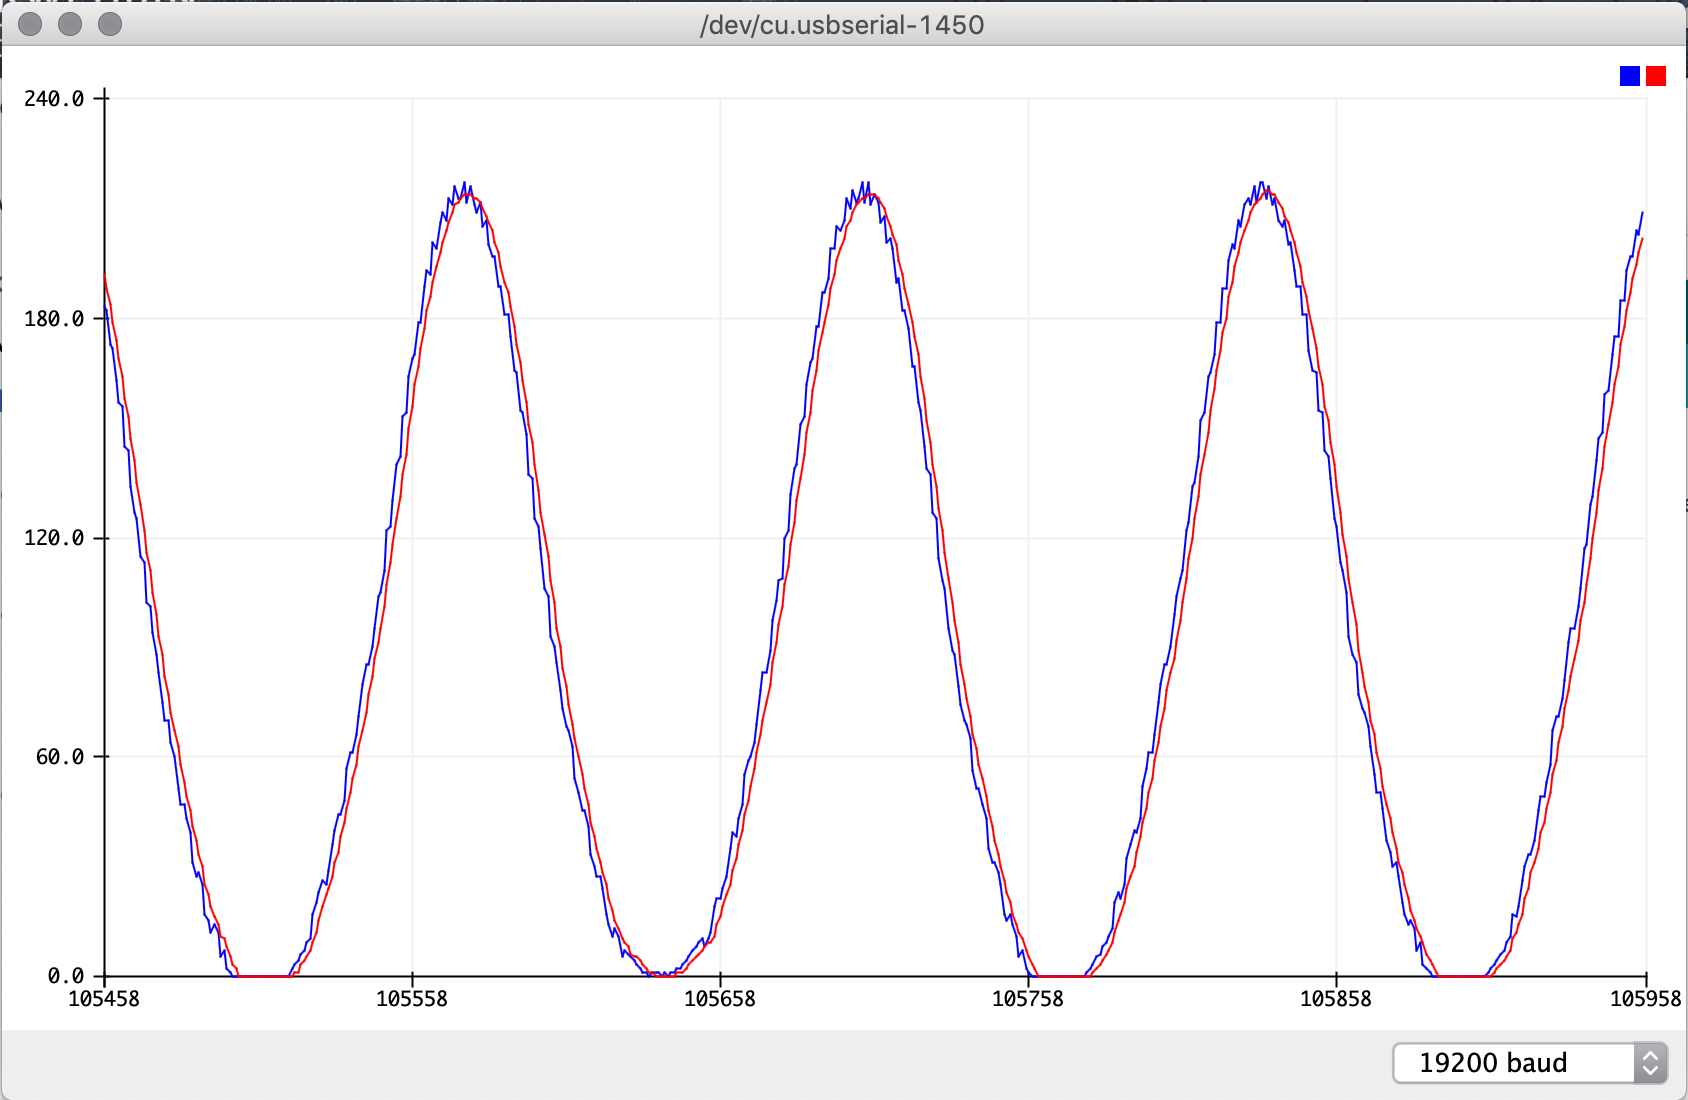
\includegraphics[width=15cm]{photos/lab/movingaverage.png}
    \caption{Moving average output (red) and noisy input (blue).}
\end{figure}
\newpage
\textbf{\underline{QUESTIONS}}
\begin{enumerate}
    \item How does the value of numavg effect the filtering of the signal? Explain what happens as the value is decreased and increased.
        \fillwithlines{1in}

    \item Compare the output of the LPF to that of the moving average filter in the plot. How are they similar? How are they different?
        \fillwithlines{1in}
        
    \item If the square waves frequency were changed to a frequency lower than the filters cutoff frequency of $f_{c} = 1kHz$, would the low pass filters output be a noiseless version of the input? Explain why or why not.
        \fillwithlines{1in}
        
    \item Explain how the averaging filter is removing the noise. Does this act as a high-pass or low-pass filter and why? 
        \fillwithlines{1in}
\end{enumerate}  

\checkoffsubsub

\section{Submission}

When you have finished all of the experiments in \textit{Section 3}, and have received a check off signature with all of the questions answered, you will begin the next lab midway through class on July 12th. If you finish on July 12th in class, do not leave. Complete the questions in the packet and bring the packet for submission in the following lab session. Submit the required codes  and document on canvas as well before the next lab session.

\end{document}